% Options for packages loaded elsewhere
\PassOptionsToPackage{unicode}{hyperref}
\PassOptionsToPackage{hyphens}{url}
%
\documentclass[
]{article}
\title{What Happened to The Birth Rate?\thanks{Replication avaliable at \url{https://doi.org/10.48152/ssrp-mbxx-jm47}. Code and data avaliable at \url{https://github.com/cuilantao/Investigation-of-falling-US-Birth-Rates-since-the-great-recession}}}
\usepackage{etoolbox}
\makeatletter
\providecommand{\subtitle}[1]{% add subtitle to \maketitle
  \apptocmd{\@title}{\par {\large #1 \par}}{}{}
}
\makeatother
\subtitle{The Great Recession and the LGBT Movement}
\author{Lantao Cui \and Huakun Shen \and Sijian Wu}
\date{27 February 2022}

\usepackage{amsmath,amssymb}
\usepackage{lmodern}
\usepackage{iftex}
\ifPDFTeX
  \usepackage[T1]{fontenc}
  \usepackage[utf8]{inputenc}
  \usepackage{textcomp} % provide euro and other symbols
\else % if luatex or xetex
  \usepackage{unicode-math}
  \defaultfontfeatures{Scale=MatchLowercase}
  \defaultfontfeatures[\rmfamily]{Ligatures=TeX,Scale=1}
\fi
% Use upquote if available, for straight quotes in verbatim environments
\IfFileExists{upquote.sty}{\usepackage{upquote}}{}
\IfFileExists{microtype.sty}{% use microtype if available
  \usepackage[]{microtype}
  \UseMicrotypeSet[protrusion]{basicmath} % disable protrusion for tt fonts
}{}
\makeatletter
\@ifundefined{KOMAClassName}{% if non-KOMA class
  \IfFileExists{parskip.sty}{%
    \usepackage{parskip}
  }{% else
    \setlength{\parindent}{0pt}
    \setlength{\parskip}{6pt plus 2pt minus 1pt}}
}{% if KOMA class
  \KOMAoptions{parskip=half}}
\makeatother
\usepackage{xcolor}
\IfFileExists{xurl.sty}{\usepackage{xurl}}{} % add URL line breaks if available
\IfFileExists{bookmark.sty}{\usepackage{bookmark}}{\usepackage{hyperref}}
\hypersetup{
  pdftitle={What Happened to The Birth Rate?},
  pdfauthor={Lantao Cui; Huakun Shen; Sijian Wu},
  hidelinks,
  pdfcreator={LaTeX via pandoc}}
\urlstyle{same} % disable monospaced font for URLs
\usepackage[margin=1in]{geometry}
\usepackage{longtable,booktabs,array}
\usepackage{calc} % for calculating minipage widths
% Correct order of tables after \paragraph or \subparagraph
\usepackage{etoolbox}
\makeatletter
\patchcmd\longtable{\par}{\if@noskipsec\mbox{}\fi\par}{}{}
\makeatother
% Allow footnotes in longtable head/foot
\IfFileExists{footnotehyper.sty}{\usepackage{footnotehyper}}{\usepackage{footnote}}
\makesavenoteenv{longtable}
\usepackage{graphicx}
\makeatletter
\def\maxwidth{\ifdim\Gin@nat@width>\linewidth\linewidth\else\Gin@nat@width\fi}
\def\maxheight{\ifdim\Gin@nat@height>\textheight\textheight\else\Gin@nat@height\fi}
\makeatother
% Scale images if necessary, so that they will not overflow the page
% margins by default, and it is still possible to overwrite the defaults
% using explicit options in \includegraphics[width, height, ...]{}
\setkeys{Gin}{width=\maxwidth,height=\maxheight,keepaspectratio}
% Set default figure placement to htbp
\makeatletter
\def\fps@figure{htbp}
\makeatother
\setlength{\emergencystretch}{3em} % prevent overfull lines
\providecommand{\tightlist}{%
  \setlength{\itemsep}{0pt}\setlength{\parskip}{0pt}}
\setcounter{secnumdepth}{5}
\newlength{\cslhangindent}
\setlength{\cslhangindent}{1.5em}
\newlength{\csllabelwidth}
\setlength{\csllabelwidth}{3em}
\newlength{\cslentryspacingunit} % times entry-spacing
\setlength{\cslentryspacingunit}{\parskip}
\newenvironment{CSLReferences}[2] % #1 hanging-ident, #2 entry spacing
 {% don't indent paragraphs
  \setlength{\parindent}{0pt}
  % turn on hanging indent if param 1 is 1
  \ifodd #1
  \let\oldpar\par
  \def\par{\hangindent=\cslhangindent\oldpar}
  \fi
  % set entry spacing
  \setlength{\parskip}{#2\cslentryspacingunit}
 }%
 {}
\usepackage{calc}
\newcommand{\CSLBlock}[1]{#1\hfill\break}
\newcommand{\CSLLeftMargin}[1]{\parbox[t]{\csllabelwidth}{#1}}
\newcommand{\CSLRightInline}[1]{\parbox[t]{\linewidth - \csllabelwidth}{#1}\break}
\newcommand{\CSLIndent}[1]{\hspace{\cslhangindent}#1}
\usepackage{subfig}
\ifLuaTeX
  \usepackage{selnolig}  % disable illegal ligatures
\fi

\begin{document}
\maketitle
\begin{abstract}
This paper is based on Kearney's paper ``The Puzzle of Falling US Birth Rates since the Great Recession.''\footnote{Original paper available at: \url{https://www.aeaweb.org/articles?id=10.1257/app.2.2.95}} (Kearney, Levine, and Pardue 2022) During the Great Recession, the US birth rate varied between a tight range of roughly 65 to 70 birth per 1000 women between the age of 15 to 44. However, after the Great Recession, the birth rate started to decline significantly, it dropped by nearly 20 percent in 13 years. In this paper, we will expand our research on multiple countries and find out whether the level of impact from recession would be correlated with the changes in the birth rate for different countries. We will also treat the rise in the LGBT community as a potential cause for the decline in birth rate and examine its effect
\end{abstract}

\hypertarget{introduction}{%
\section{Introduction}\label{introduction}}

The Great Recession has been a worldwide crisis that reconstructed the economy and was deep, synchronous and global. Canadian GDP dropped by 3.3 percent, US GDP by close to 4 percent, that of the Euro area by 5 percent, and that of Japan by more than 8 percent. The impact on international trade has been severe that all G20 countries experienced serious reductions in trade(Michael Hart 2010). Apart from the economic impact, the great recession also had a negative impact on the country's birth rate.

In the United States, unemployment rates, mortgage foreclosures, and poverty rates rose while housing values fell, but the extent of these changes varied widely across local areas. Another impact from the depressed economic condition is delayed childbearing, and others to hasten it. The fertility rate declined at the national level, dropping from a recent high in 2007 of 69.5 births per 1,000 women aged 15 to 44, to 63.2 for 2012.1 There was, however, great variation by state, age, and ethnicity, with younger and Hispanic women showing disproportionate decreases(Christine Percheski 2017). The significant consequence on fertility rate would make us wonder how severe is America being affected by the great recession. However, by comparing currency devaluations, equity market declines, and rising sovereign bond spreads, the U.S. is the third less affected country(URI DADUSH 2009).

Prior research suggests that stress may be linked to riskier sexual activity. Financial hardship and poverty can negatively affect cognitive function, and shorten the time horizons over which individuals make cost-benefit determinations. Alternatively, fertility may be unaffected by economic conditions if cultural norms related to the context and timing of births are particularly influential. For example, non-marital births are more socially consequential for some racial and ethnic groups, and in some geographic areas. For some individuals, these social norms may outweigh any economic considerations(Christine Percheski 2017). The same consideration of religious belief could also be applied to other countries.

As mentioned by Kearney, Levine, and Pardue (2022), the basic approach to many economic problems is maximizing utility. This approach recognized that children bring people utility but also comes with associated costs including time and money. This approach to modeling the decision to have a child leads to standard predictions of price and income effects. Direct consideration of costs could be like housing and medical care. Other times the price effect is indirect, as the opportunity cost of a woman's time. Holding prices and quality constant, an increase in income will lead people to choose to have more children. This positive relationship between income and births may come as a surprise to some readers, given the negative relationship between birth rates and income or per-capita GDP observed over time and place(Kearney, Levine, and Pardue 2022). However, this is enough for us to consider whether the birth rates are worldwide affected in the same negative direction after the Great Recession.

Another thing that might have affected the fertility rate is the rise of the LGBT community, the LGBT activity started in the 1920s and had huge progress after the 2000s. A lot of laws that prohibited homosexual relationships were lifted and homosexual couples can get married legally and adopt kids, there is also propaganda that encourages homosexuality.

In this paper, we will investigate the effect of the Great Recession on the birth rate in different countries, and we will also explore the effect of the LGBT movement on the birth rate.

\hypertarget{data}{%
\section{Data}\label{data}}

We started our analysis by using R (R Core Team 2020), dplyr(Wickham et al. 2021), tidyverse(Wickham et al. 2019). Graphs are generated using ggpubr(Kassambara 2020) and ggplot2(Wickham 2016).

\hypertarget{data-source}{%
\subsection{Data Source}\label{data-source}}

Part of our data are from the NCHS(National Center for Health Statistics)({``NVSS - Birth Data''} 2022), in particular, we acquired the US birth rate data for the past 40 years, Figure \ref{fig:fig-past-40-years} shows the US birth rate from 1980 - 2020, as we can see, the birth rate declined significantly after 2007, which is the time of the Great Recession. We also generated data from U.S. Birth Rate 1950-2022(Trends 2022). We selected the top 3 countries that are affected most and least by the Great Recession according to rankings determined by comparing currency devaluations, equity market declines, and rising sovereign bond spreads. These measures tend to track developments in the real economy during times of economic crisis when financial strain handicaps consumption, investment, and in many cases government spending, which limits GDP and employment growth(URI DADUSH 2009). TODO: ADD DATA SOURCE AND BREIFLY TALK ABOUT IT

\hypertarget{data-characteristics}{%
\subsection{Data Characteristics}\label{data-characteristics}}

The NCHS data source is very detailed, it contains a lot of demographic and geographic information. For example, for each birth, the data set records the race of the father and the mother, this can help us to analyze the birth rate among different race groups. It also contains the age of the mother and father, this can be really helpful if we want to examine the trend of teenager pregnancy.

\begin{figure}
\centering
\includegraphics{paper_files/figure-latex/fig-past-40-years-1.pdf}
\caption{\label{fig:fig-past-40-years}US Birth Rate in the past 40 years}
\end{figure}

\hypertarget{results}{%
\section{Results}\label{results}}

\hypertarget{global-comparison-of-fertility-rate-under-the-great-recession}{%
\subsection{Global Comparison of Fertility Rate Under The Great Recession}\label{global-comparison-of-fertility-rate-under-the-great-recession}}

It shows that although the United States is at the epicenter of the global economic crisis, it is one of the countries least affected by the financial fallout. Large industrialized nations like the United States, Japan, and Germany have benefited from increasing global demand for relatively stable economies in which to invest. Instead, it is several developing countries, notably those with vulnerable capital accounts and weak macroeconomic fundamentals, that are experiencing severe economic downturns disproportionate to their roles in the crisis(URI DADUSH 2009).

\begin{figure}
\centering
\includegraphics{paper_files/figure-latex/least-affected-1.pdf}
\caption{\label{fig:least-affected}Births per 1000 People of Top Least Affected Countries}
\end{figure}

Figure \ref{fig:least-affected} shows the changes of births per 1000 people of China, Japan, the U.S, and South Africa since 1950 with the prediction for the future. The births rates of China and South Africa were obviously higher than the U.S. and Japan. However, around the year of recession, the birth rate of China and Japan dropped even harder than the U.S. on the absolute level that is lower than 10 births per 1000 people.

\begin{figure}
\centering
\includegraphics{paper_files/figure-latex/most-affected-1.pdf}
\caption{\label{fig:most-affected}Births per 1000 People of Top Most Affected Countries}
\end{figure}

Figure \ref{fig:most-affected} shows the changes of births per 1000 people of Ukraine, Argentina, Hungary, Poland since 1950 with prediction for the future. All these most affected countries have lower initial births rate than those least affected countries. However, the levels of births per 1000 people were similar to those least affected countries around recession except Argentina. Ukraine, Hungary, and Poland also showed a potential increase after recession but continued to decline afterwards.

\textless\textless\textless\textless\textless\textless\textless{} HEAD
\#\# Effect of LGBT movement
=======
We do observe declinations of world-wide birth rate despite of the impact level from recession. From the economic perspective, the countries who are least affected tend to have a stronger resistance to recession but not necessarily developed countries. While the most affected countries are mostly developing countries, they experienced a more significant plummet as percentage. It is also intriguing that the long-term births per 1000 people tend to converge to 10 for all countries mentioned above. However, the countries have higher resistance tend to delay the convergence which may derived from stronger economic status. Overall, the Great Recession was a turning point not only for the U.S. but also the whole world in the context of birth rate. The Great Recession may not be the direct cause of the world-wide declination in birth rates but it indeed provided an opportunity and provoked the desire for people to reconsider personal priorities with changed perspective of the society.

\hypertarget{effect-of-lgbt-movement}{%
\subsection{Effect of LGBT Movement}\label{effect-of-lgbt-movement}}

\begin{quote}
\begin{quote}
\begin{quote}
\begin{quote}
\begin{quote}
\begin{quote}
\begin{quote}
dce133630df142da93e120527ceec753178efac5
\end{quote}
\end{quote}
\end{quote}
\end{quote}
\end{quote}
\end{quote}
\end{quote}

The percentage of LGBT (and many other gender identities) population has risen in recent years in the US, probably related to propaganda and political correctness.

Since there is not much data for other genders, and LGBT are the majorities, we will focus on LGBT population and the potential effect they bring to birth rate.

LGBT is the acronym of the following 4 gender identities, \textbf{L} for Lesbian, \textbf{G} for gay, \textbf{B} for bisexual, \textbf{T} for transgender. By definition, these genders should have a much lower birth rate than that of the heterosexual as normal births of human must depend on a male and a female.
Figure \ref{fig:fig-gender-raising-children-distribution} (b) shows the percentage of LGBT population that raise children. 71\% of the LGBT population don't raise children.
Then changes in birth rate and changes in LGBT population should have a negative proportional relationship (i.e.~Growth in LGBT population leads to lower birth rate).
Thus, the population changes in these population are very likely to make an impact on the birth rate of the US.

If we assume the simpliest scenario where we ignore race, gender distribution (equal percentage of male and female) and all other factors, and assume that no LGBT or same-sex-couple population give birth to a child, then there would be a perfect correlation (perfectly proportional) between LGBT population change and birth rate (i.e.~an \(x\%\) increase in LGBT population could lead to an \(x\%\) decrease in birth rate). Let's define \(\phi = \frac{\Delta Birth Rate}{\Delta LGBTPopulation}\) and call \(\phi\) the BirthRate-LGBT coefficient for convenience. Basically, lower BirthRate-LGBT coefficient means lower birth rate while holding LGBT population constant. If we take other factors into account, the impact to birth rate could be even larger (i.e.~\(\phi<-1\)).

\begin{figure}
\subfloat[LGBT Gender Distribution\label{fig:fig-gender-raising-children-distribution-1}]{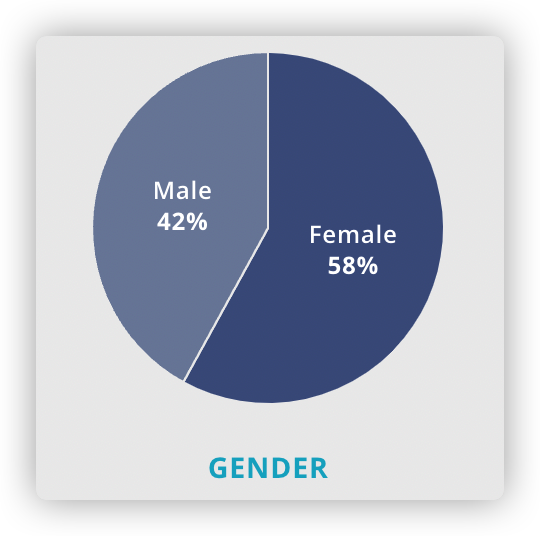
\includegraphics[width=.33\linewidth]{./images/LGBT-Gender-distribution} }\subfloat[LGBT Percentage Raising Children\label{fig:fig-gender-raising-children-distribution-2}]{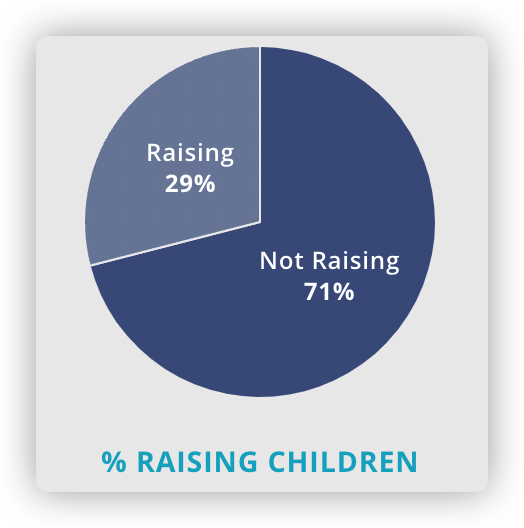
\includegraphics[width=.33\linewidth]{./images/LGBT-percentage-raising-children} }\subfloat[Same Sex Couple Gender Distribution\label{fig:fig-gender-raising-children-distribution-3}]{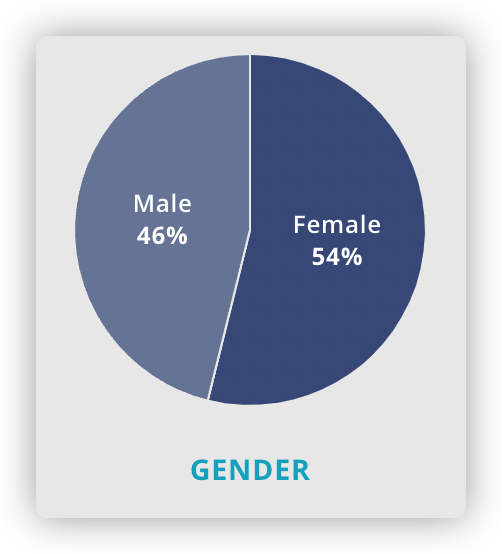
\includegraphics[width=.33\linewidth]{./images/same-sex-couple-gender-distribution} }\caption{Gender Distribution and Percentage Raising Children Distribution}\label{fig:fig-gender-raising-children-distribution}
\end{figure}

Figure \ref{fig:fig-gender-raising-children-distribution} shows the gender distribution of LGBT and Same Sex Couple as well as well as the percentage raising children (n.d.).
Figure \ref{fig:fig-gender-raising-children-distribution} (a) and Figure \ref{fig:fig-gender-raising-children-distribution} (c) clearly shows that more females are non-heterosexual than male are (n.d.).
This could cause a lower BirthRate-LGBT coefficient on birth rate as only females are able to give births (in normal situations).

\begin{figure}
\subfloat[Same Sex Couple State Density\label{fig:fig-density-state-1}]{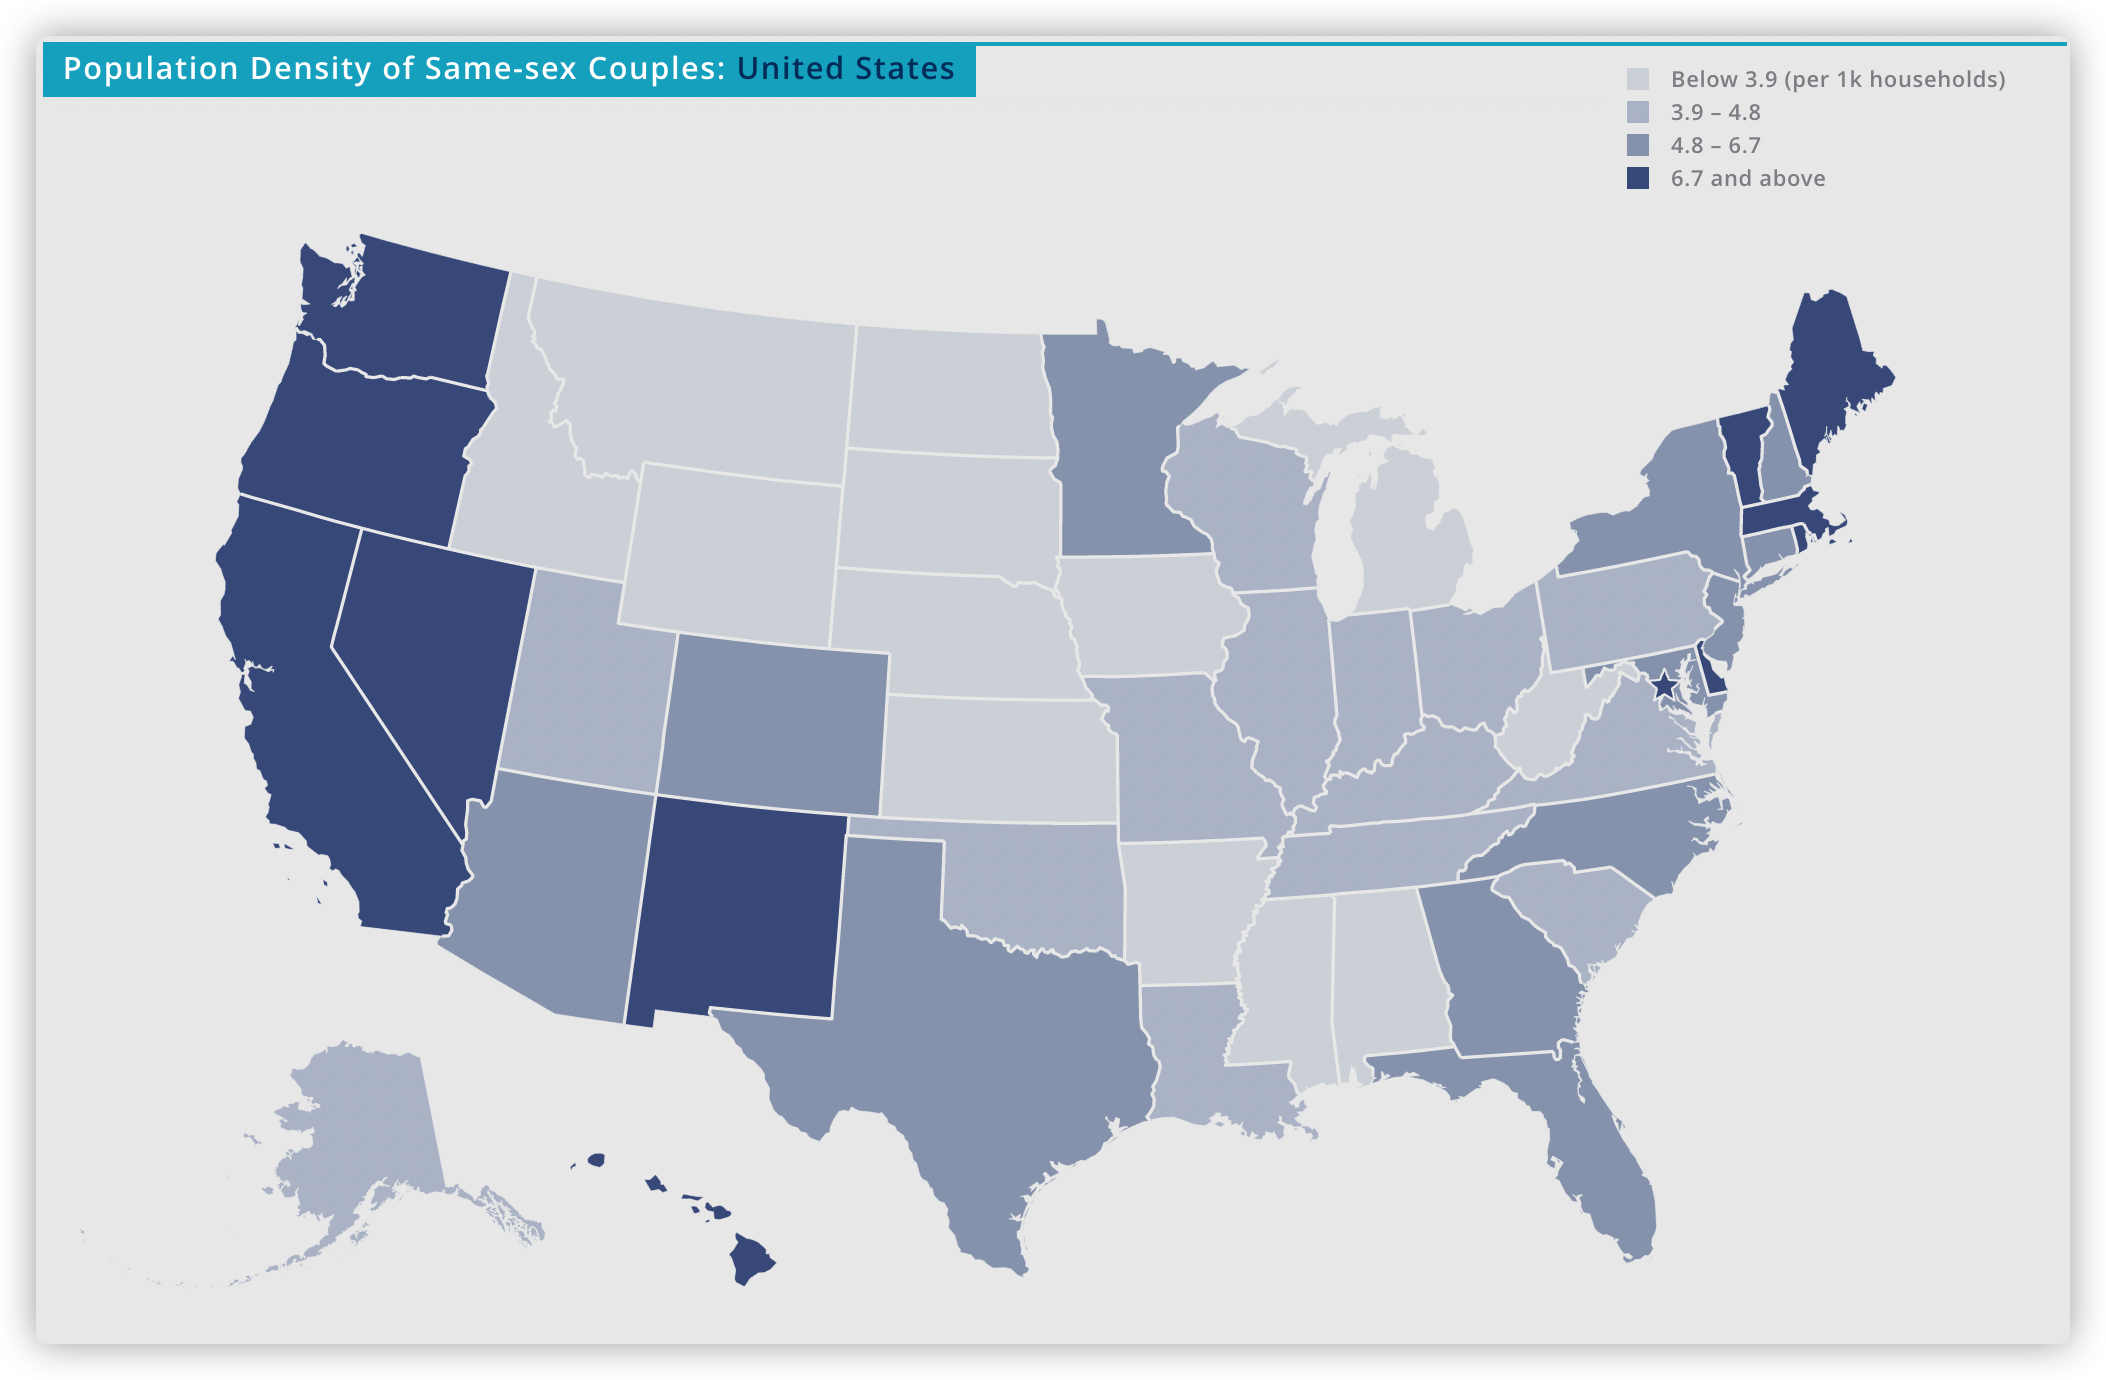
\includegraphics[width=.49\linewidth]{./images/same-sex-couple-state-density} }\subfloat[LGBT State Density\label{fig:fig-density-state-2}]{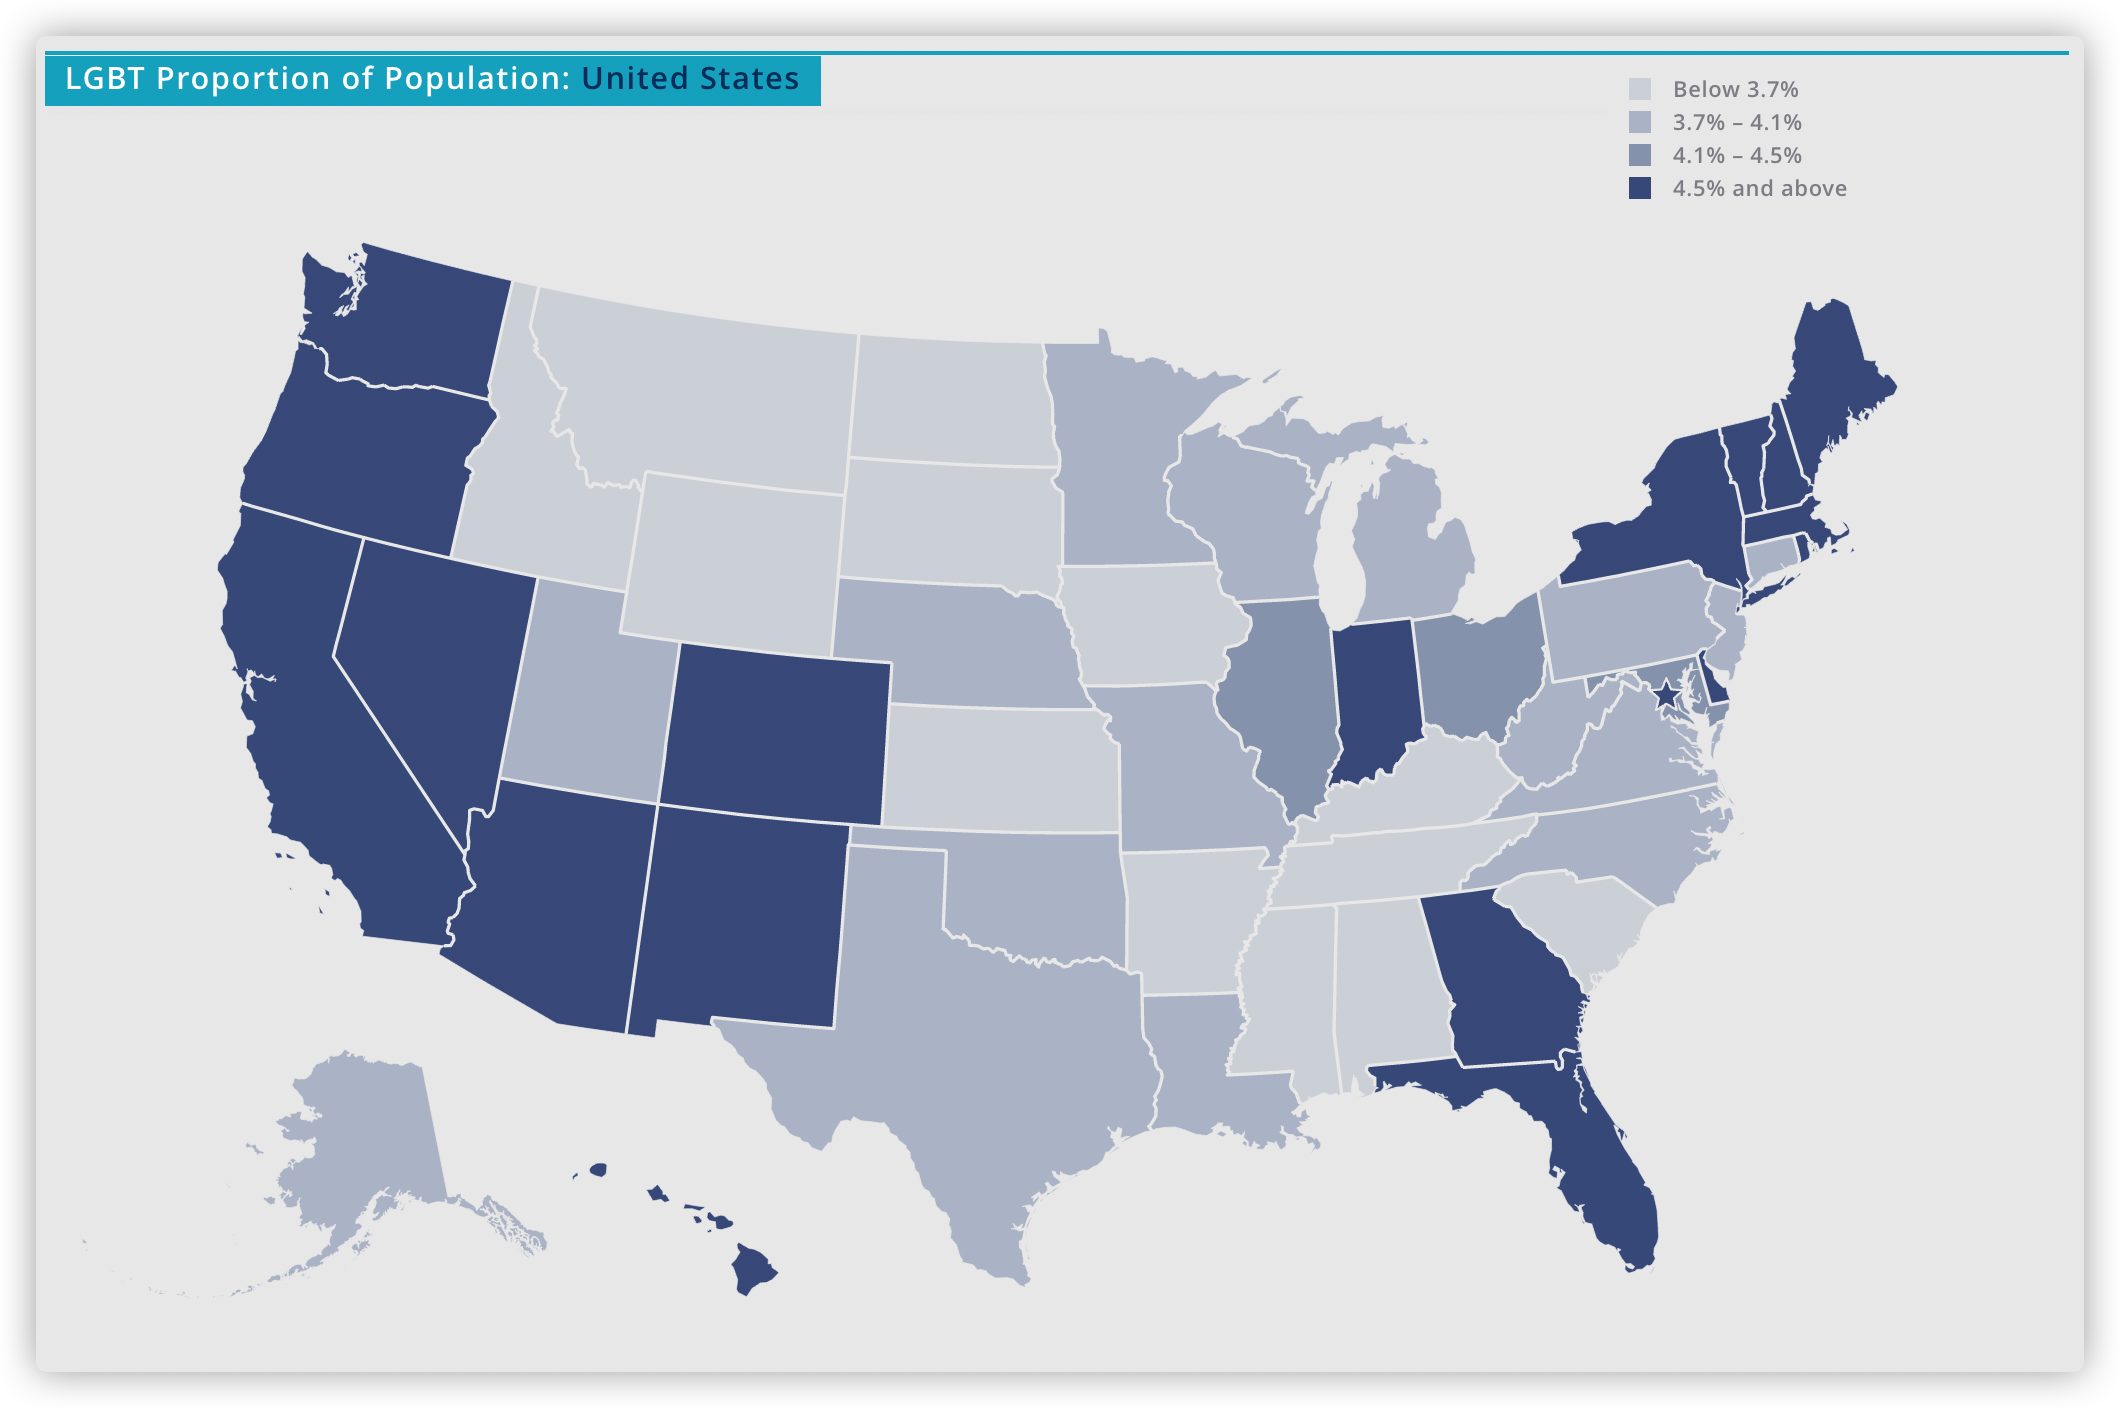
\includegraphics[width=.49\linewidth]{./images/LGBT-state-density} }\newline\subfloat[Birth Rate Distribution by State\label{fig:fig-density-state-3}]{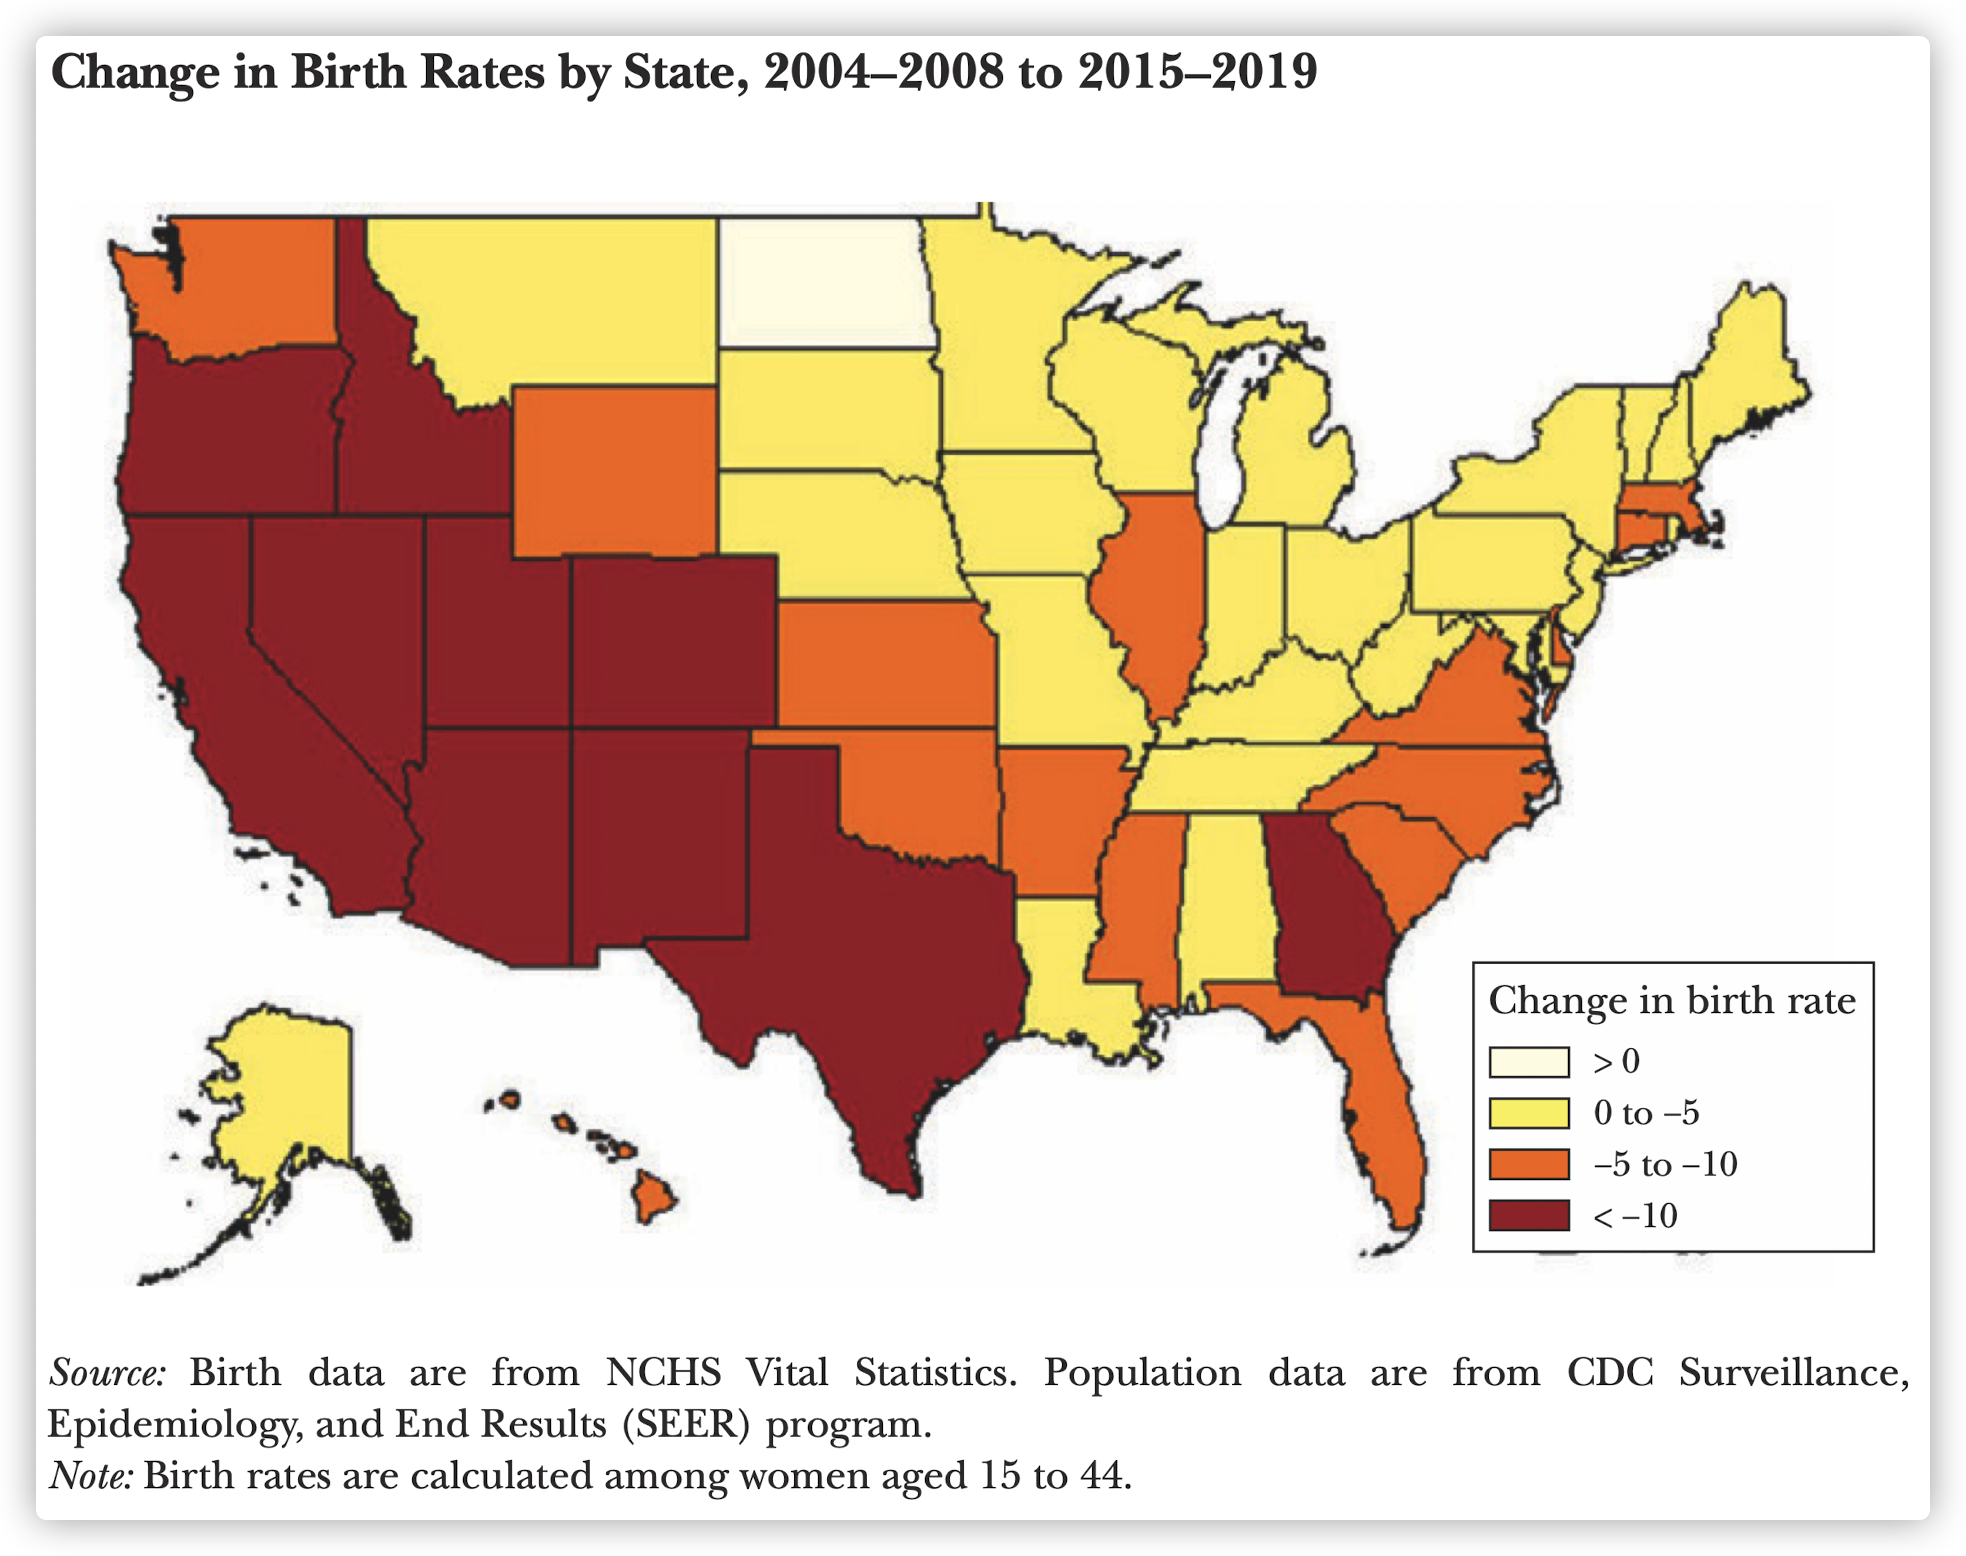
\includegraphics[width=.49\linewidth]{./images/state-birth-rate-distribution} }\caption{Density by State}\label{fig:fig-density-state}
\end{figure}

Figure \ref{fig:fig-density-state} (a) and Figure \ref{fig:fig-density-state} (b) shows the population density of Same Sex Couple and LGBT by States in the US (n.d.).
Figure \ref{fig:fig-density-state} (Kearney, Levine, and Pardue 2022) (c) shows the birth rate distribution by State in the US. Darker color means higher density or larger negative change in birth rate (n.d.). From these plots we can see that the states with higher LGBT density and same sex couples generally have larger negative change in birth rate. States on the west generally have darker color in all three plots. We cannot conclude whether LGBT population has a large or direct impact on US birth rate based on these plots yet, but there should be some correlation between birth rate and gender identity of Americans.

\begin{figure}

{\centering \subfloat[Same Sex Couple Race Distribution\label{fig:fig-race-distribution-1}]{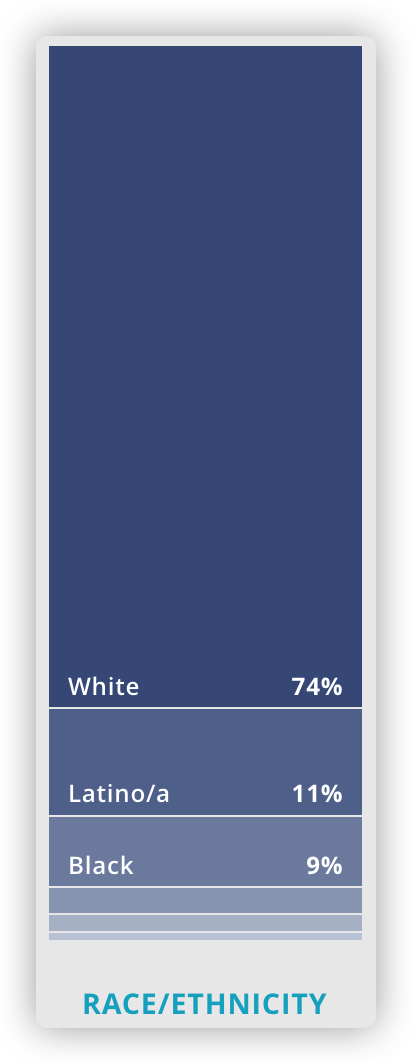
\includegraphics[width=.30\linewidth]{./images/same-sex-couple-race-distribution} }\subfloat[LGBT Race Distribution\label{fig:fig-race-distribution-2}]{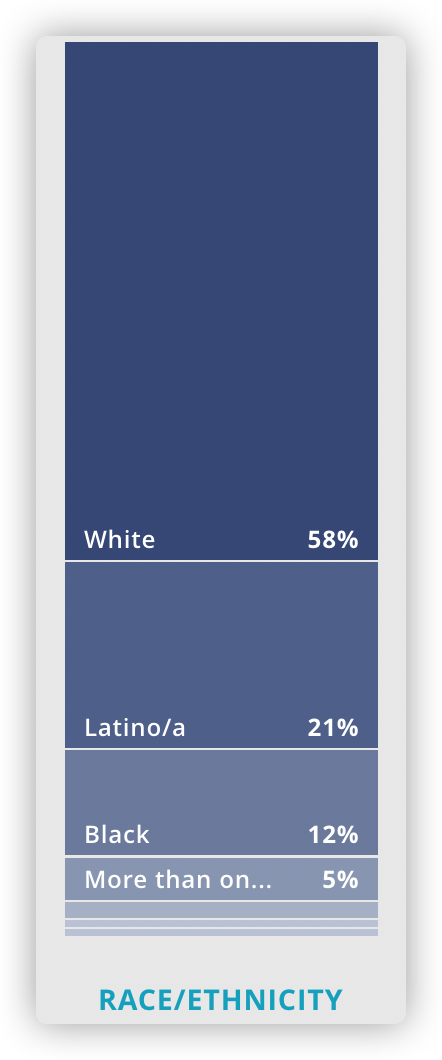
\includegraphics[width=.30\linewidth]{./images/LGBT-race-distribution} }

}

\caption{Race Distribution}\label{fig:fig-race-distribution}
\end{figure}

From \ref{fig:fig-race-distribution} we can see that White population takes up the majority of the population of LGBT (58\%) and Same Sex Couple (74\%) (n.d.). White is also the majority of the population in the US ({``U.s. Census Bureau Quickfacts: United States,''} n.d.), around 76.3\% of the total population. Thus, larger LGBT population could lead to an even larger decrease in birth rate (\(\phi<-1\), lower BirthRate-LGBT coefficient).

\begin{figure}

{\centering \subfloat[Same Sex Couple Race Distribution\label{fig:fig-age-distribution-1}]{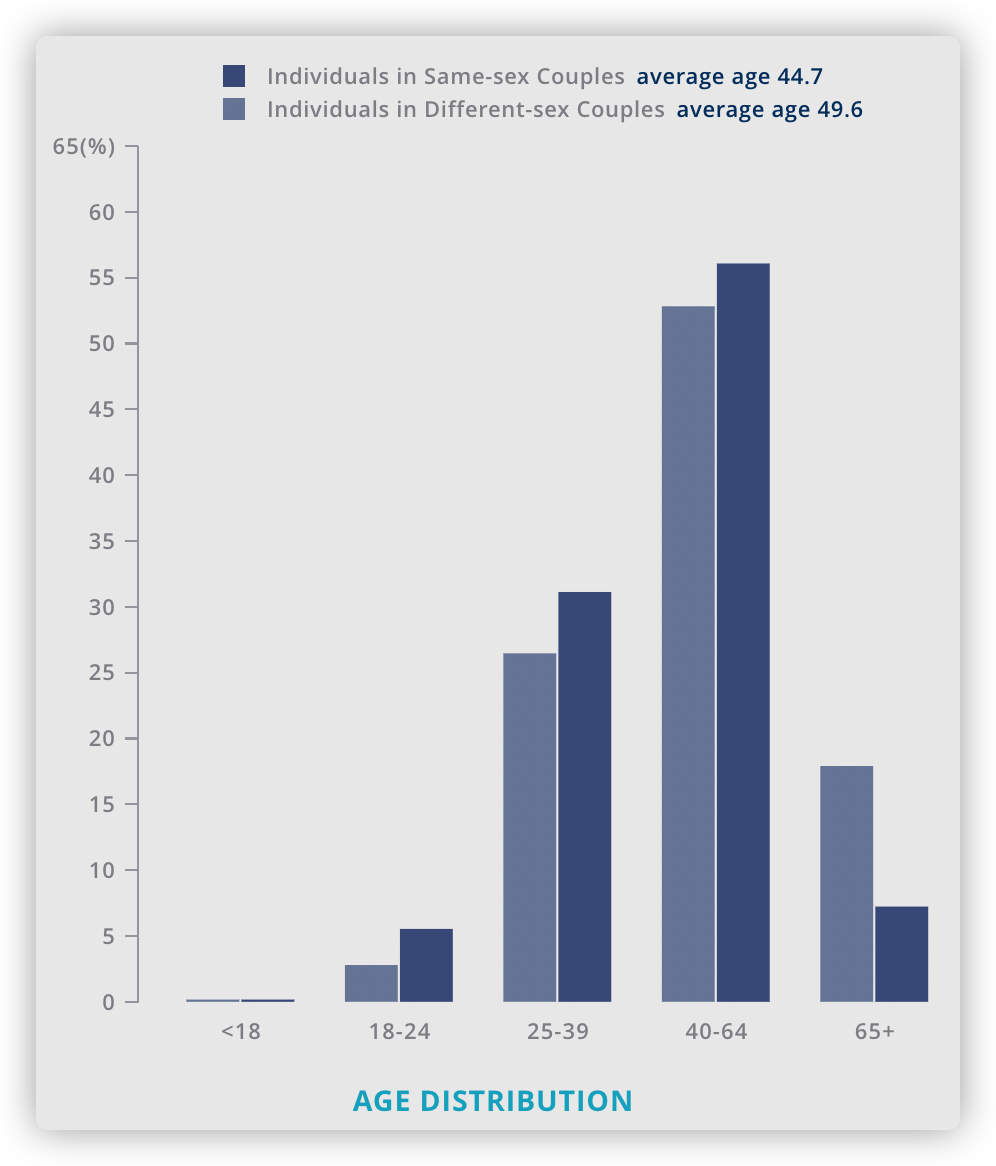
\includegraphics[width=.40\linewidth]{./images/same-sex-couple-age-distribution} }\subfloat[LGBT Race Distribution\label{fig:fig-age-distribution-2}]{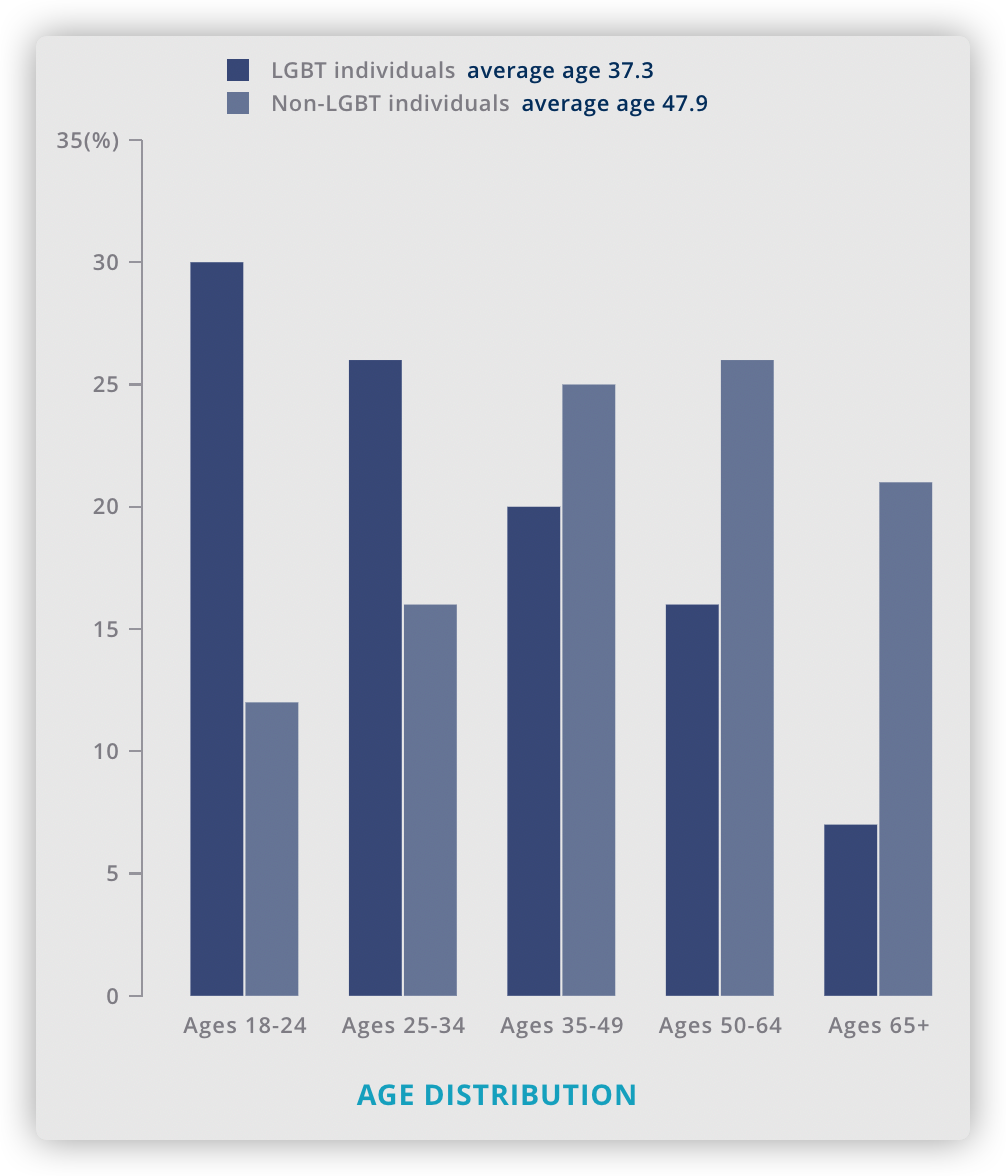
\includegraphics[width=.40\linewidth]{./images/LGBT-age-distribution} }

}

\caption{LGBT and Same Sex Couple Age Distribution}\label{fig:fig-age-distribution}
\end{figure}

From \ref{fig:fig-age-distribution} (a) we can see that most same sex couples fall in the age group 25-64 (n.d.). This period overlaps with the majority of the childbearing age. From \ref{fig:fig-age-distribution} (b) (n.d.), we can see that LGBT population decreases as age increases starting from the age or 18, which is the beginning of women's childbearing age. Around 90\% of the LGBT population have their age between 18 and 64, which covers almost all of the child bearing ages. These 2 evidences also indicate that, growth of LGBT population could lead to a larger decrease in birth rate (\(\phi < -1\), lower BirthRate-LGBT coefficient).

With these information, we can conclude that the growth of LGBT population is able to cause a negative change in birth rate.

\begin{figure}

{\centering 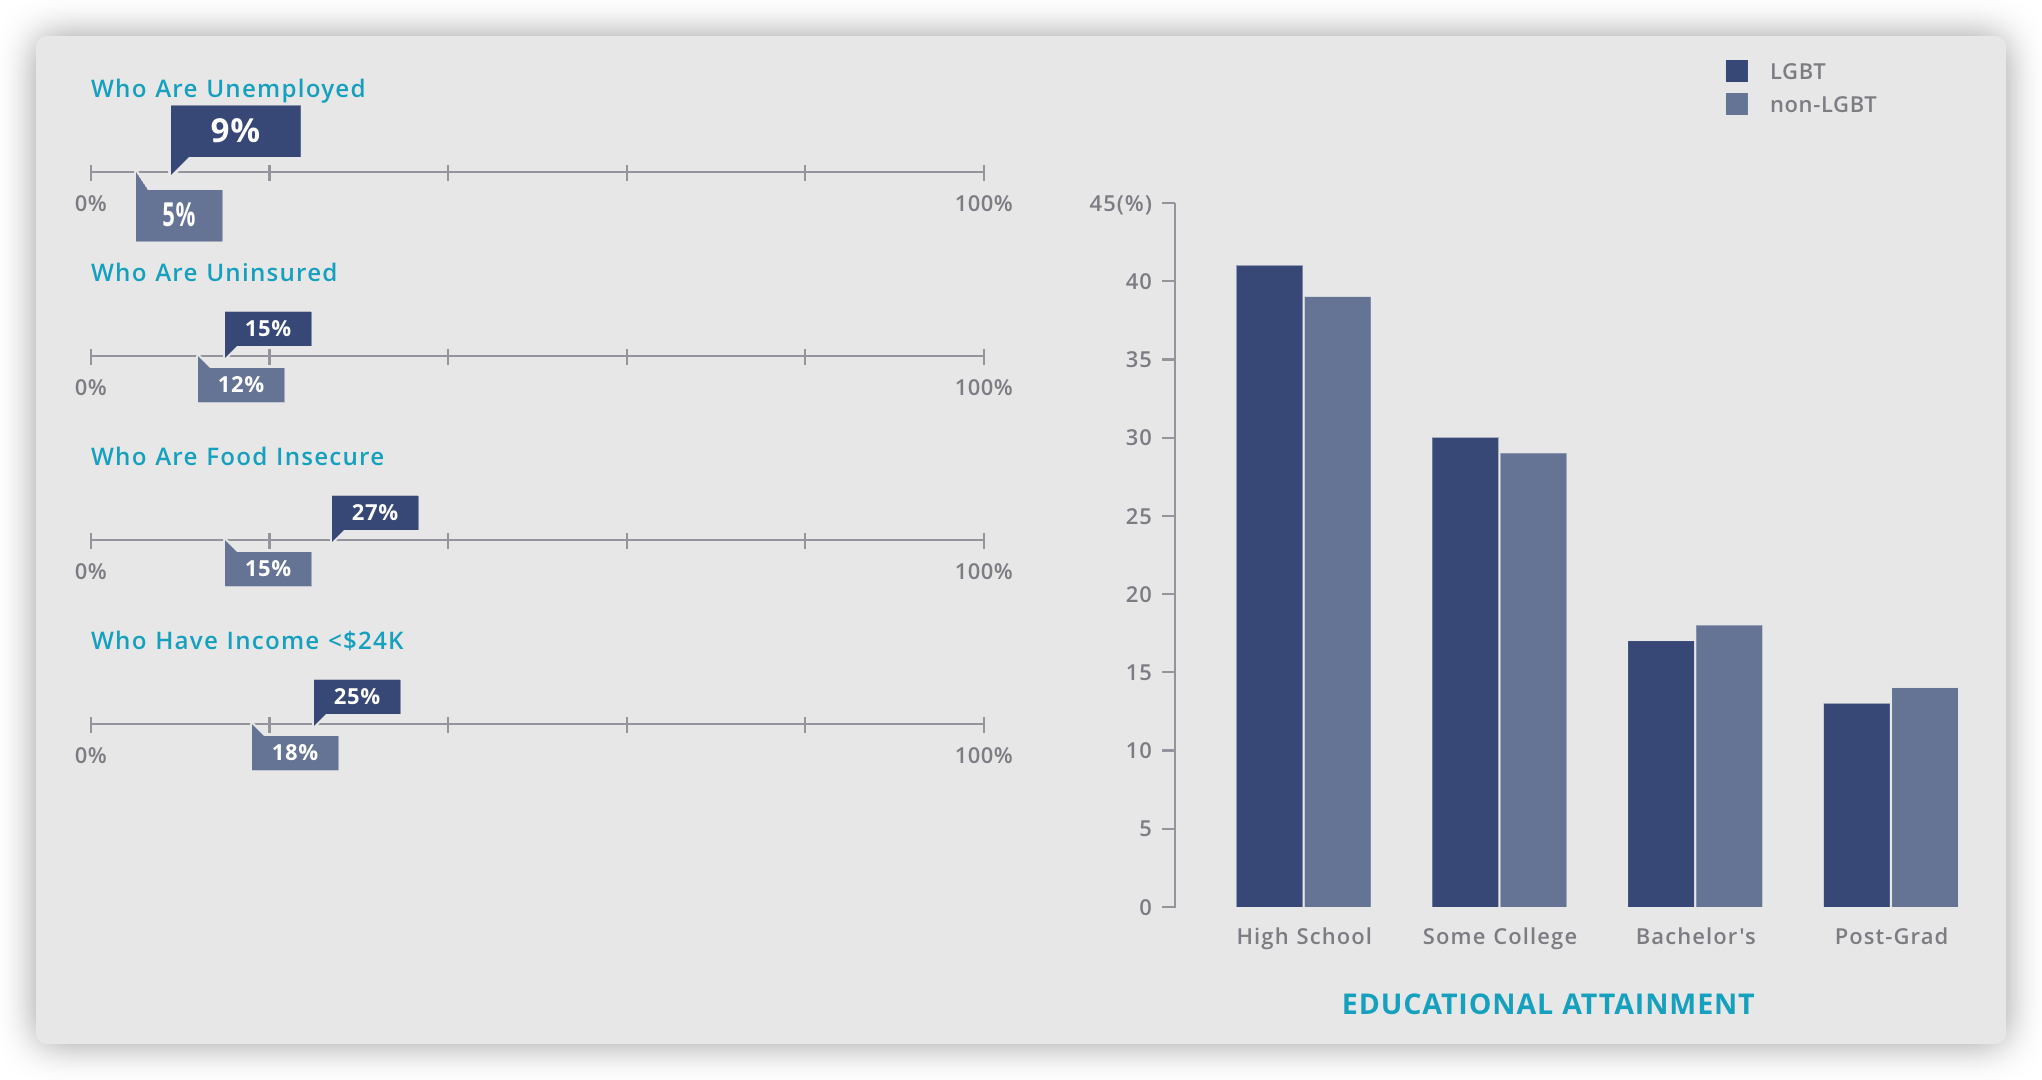
\includegraphics[width=.80\linewidth]{./images/LGBT-socioeconomic-indicators} 

}

\caption{Socioeconomic Indicators}\label{fig:fig-LGBT-socioeconomic-indicators}
\end{figure}

Figure \ref{fig:fig-LGBT-socioeconomic-indicators} shows some socioeconomic indicators classified by sexual orientation (LGBT or not), such as employment status, income level education level, and whether or not being insured and food insecure (n.d.). Darker color represents LGBT, lighter color represents non-LGBT.
From the plots, we can extract some socioeconomic indicators of LGBT. Comparing to non-LGBT population, LGBT population might be more likely to be unemployed, uninsured, being food insecure, having a low income (lower then \$24k), and having a lower education level (percentage of LGBT population with Bachelor's or post-grad degree is slightly lower than that of the percentage of non-LGBT population). It's not rigorous to conclude that LGBT are more

\hypertarget{cohort-effect}{%
\subsection{Cohort Effect}\label{cohort-effect}}

\begin{figure}
\centering
\includegraphics{paper_files/figure-latex/cohort-plot-1.pdf}
\caption{\label{fig:cohort-plot}Children Ever Born by Mother Age and Birth Cohort}
\end{figure}

Research has shown that cohort effects may have contributed to the declines of birth rate in the US(Kearney, Levine, and Pardue 2022).
``Period effects reflect changes that affect everyone at a point in time, whereas cohort effects reflect changes across people born or raised in different years.''(Kearney, Levine, and Pardue 2022).

We reproduced the plot showing Fertility Rate vs Mother's age from (Kearney, Levine, and Pardue 2022) in Figure \ref{fig:cohort-plot}. This plot is basically showing the fertility rate of women in different ages across 6 generations.
It's quite obvious that the 3 oldest cohorts (generations) have similar and higher fertility rates comparing to that of the 3 younger cohorts (generations).The 3 younger cohorts also have lower and lower fertility rate as their birthday moves forward (younger generation -\textgreater{} lower fertility rate).

\begin{figure}
\centering
\includegraphics{paper_files/figure-latex/fig-parity-1.pdf}
\caption{\label{fig:fig-parity}Parity (ages 15-44)}
\end{figure}

Figure \ref{fig:fig-parity} is a replication of a plot showing trends in births by ``parity'' (referring to the number of children for a given woman) from (Kearney, Levine, and Pardue 2022). First and second births declined a lot since 2007, but the trend lines for third and higher order births are comparatively flat.
The women giving their 3rd and 4th births are most likely an older cohort than the cohorts giving their 1st and 2nd births. Again, this is another evidence showing the impact brought by cohort effects.

\begin{figure}

{\centering 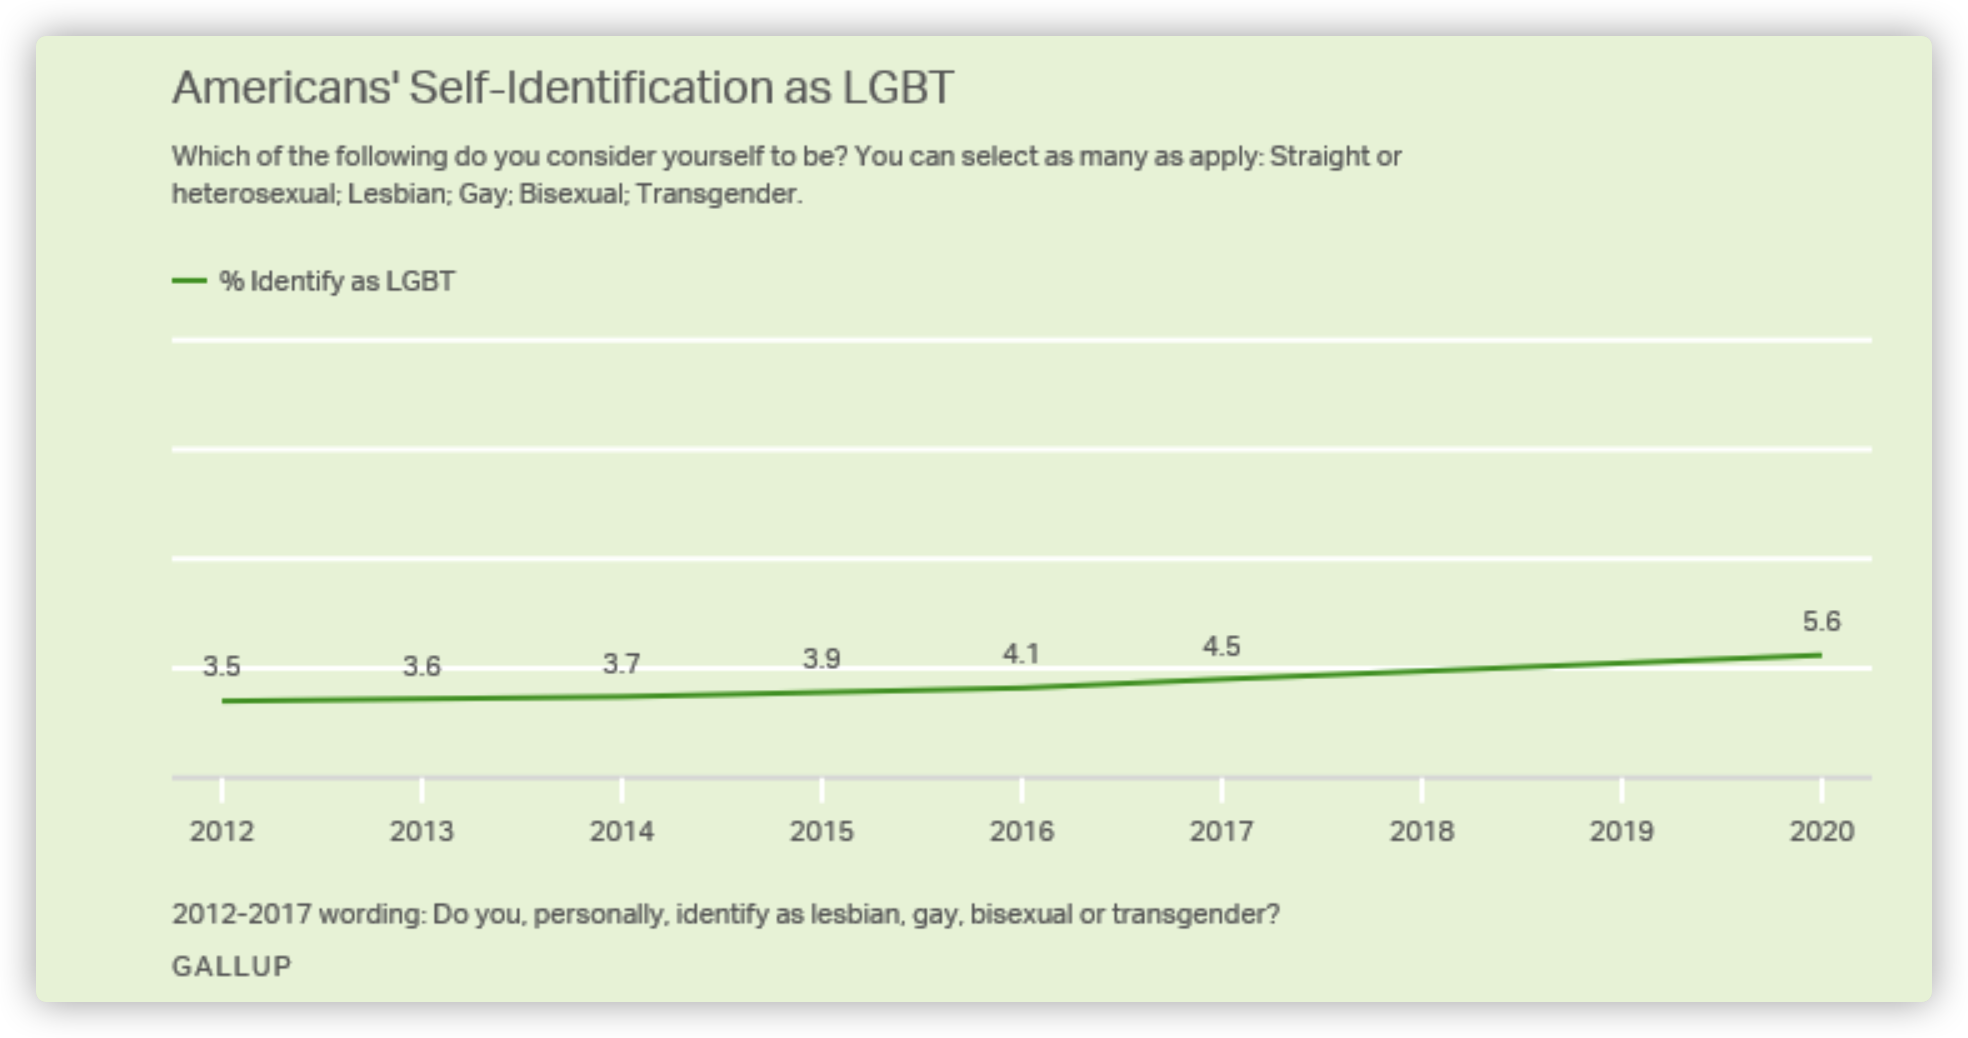
\includegraphics[width=.80\linewidth]{./images/US-LGBT-percent-trend} 

}

\caption{Socioeconomic Indicators}\label{fig:fig-lgbt-trend-by-year}
\end{figure}

\begin{figure}

{\centering 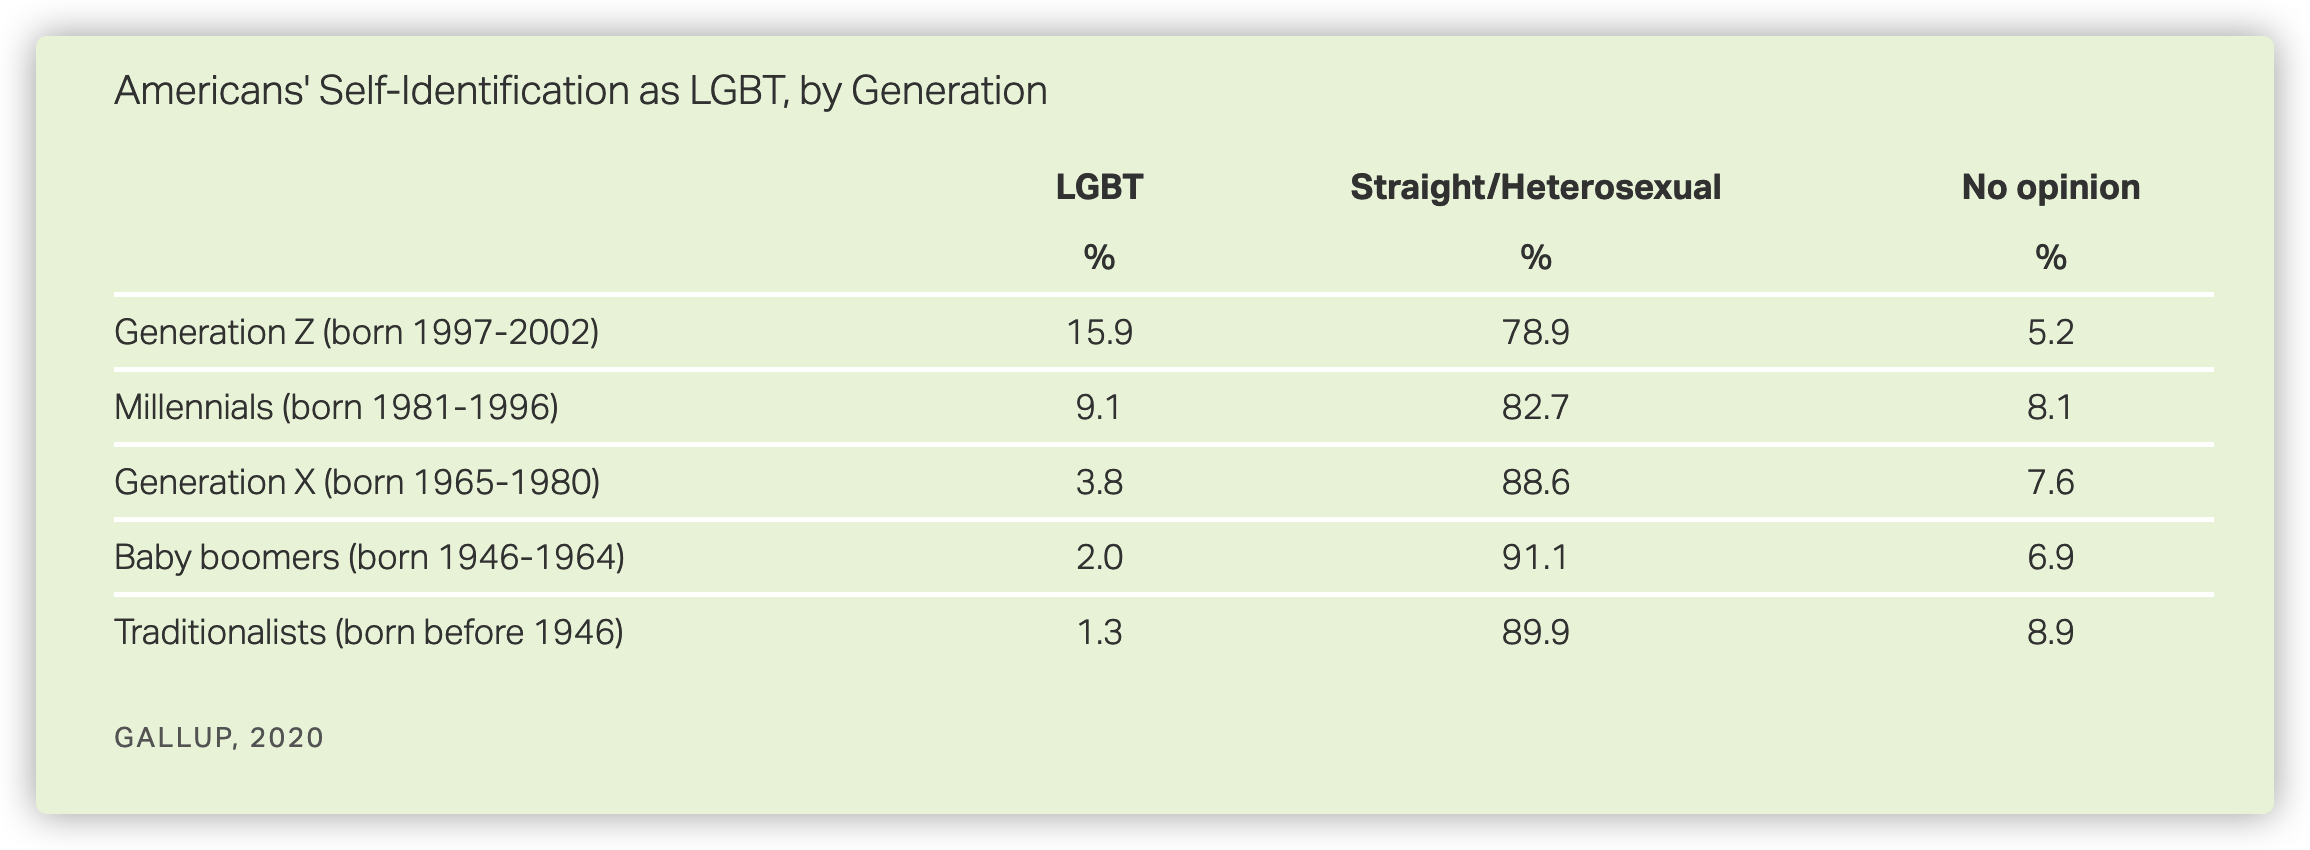
\includegraphics[width=.80\linewidth]{./images/LGBT-percentage-by-generation} 

}

\caption{Socioeconomic Indicators}\label{fig:fig-lgbt-by-generation}
\end{figure}

\hypertarget{lgbt-and-cohort-effect}{%
\subsection{LGBT and Cohort Effect}\label{lgbt-and-cohort-effect}}

Figure \ref{fig:fig-lgbt-trend-by-year} shows the trend of LGBT population percentage in total population.
There is an obvious increasing trend (i.e.~higher percentage of the US population are becoming LGBT) (Jones 2021).
Figure \ref{fig:fig-lgbt-by-generation} shows the percentage of LGBT population trend in different generations (Jones 2021).
We can also see an increasing trend of LGBT population percentage (younger generations are more and more likely to become LGBT).
This provides more evidence that cohort effects and the growth of LGBT population may have contributed a lot to the declines of birth rate in the US in recent years.

\hypertarget{discussion}{%
\section{Discussion}\label{discussion}}

\hypertarget{global-comparison}{%
\subsection{Global Comparison}\label{global-comparison}}

We do observe declination of world-wide birth rate despite of the impact level from recession. From the economic perspective, the countries who are least affected tend to have a stronger resistance to recession but not necessarily developed countries. While the most affected countries are mostly developing countries, they experienced a more significant plummet as percentage. It is also intriguing that the long-term births per 1000 people tend to converge to 10 for all countries mentioned above. However, the countries have higher resistance tend to delay the convergence which may derived from stronger economic status. Overall, the Great Recession was a turning point not only for the U.S. but also the whole world in the context of birth rate. The Great Recession may not be the direct cause of the world-wide declination in birth rates but it indeed provided an opportunity and provoked the desire for people to reconsider personal priorities with changed perspective of the society.

\newpage

\hypertarget{references}{%
\section*{References}\label{references}}
\addcontentsline{toc}{section}{References}

\hypertarget{refs}{}
\begin{CSLReferences}{1}{0}
\leavevmode\vadjust pre{\hypertarget{ref-will_institute}{}}%
n.d. \emph{The Williams Institute}. \url{https://williamsinstitute.law.ucla.edu/visualization/lgbt-stats/\#density}.

\leavevmode\vadjust pre{\hypertarget{ref-fertility}{}}%
Christine Percheski, Rachel Kimbro. 2017. {``How Did the Great Recession Affect Fertility?''} \url{https://www.irp.wisc.edu/publications/focus/pdfs/foc302g.pdf}.

\leavevmode\vadjust pre{\hypertarget{ref-us_lgbt_trend}{}}%
Jones, Jeffrey M. 2021. {``LGBT Identification Rises to 5.6.''} \emph{Gallup.com}. Gallup. \url{https://news.gallup.com/poll/329708/lgbt-identification-rises-latest-estimate.aspx}.

\leavevmode\vadjust pre{\hypertarget{ref-ggpubr}{}}%
Kassambara, Alboukadel. 2020. \emph{Ggpubr: 'Ggplot2' Based Publication Ready Plots}. \url{https://CRAN.R-project.org/package=ggpubr}.

\leavevmode\vadjust pre{\hypertarget{ref-cite_original}{}}%
Kearney, Melissa S., Phillip B. Levine, and Luke Pardue. 2022. {``The Puzzle of Falling US Birth Rates Since the Great Recession.''} \emph{Journal of Economic Perspectives} 36 (1): 151--76. \url{https://doi.org/10.1257/jep.36.1.151}.

\leavevmode\vadjust pre{\hypertarget{ref-recession}{}}%
Michael Hart, Bill Dymond. 2010. {``The Great Recession and International Trade.''} \url{https://policyoptions.irpp.org/magazines/g8g20/the-great-recession-and-international-trade/}.

\leavevmode\vadjust pre{\hypertarget{ref-nvss}{}}%
{``NVSS - Birth Data.''} 2022. \emph{Centers for Disease Control and Prevention}. Centers for Disease Control; Prevention. \url{https://www.cdc.gov/nchs/nvss/births.htm}.

\leavevmode\vadjust pre{\hypertarget{ref-r}{}}%
R Core Team. 2020. \emph{R: A Language and Environment for Statistical Computing}. Vienna, Austria: R Foundation for Statistical Computing. \url{https://www.R-project.org/}.

\leavevmode\vadjust pre{\hypertarget{ref-birthrate}{}}%
Trends, Macro. 2022. {``Birth Rate 1950-2022.''} \url{https://www.macrotrends.net/countries/USA/united-states/birth-rate}.

\leavevmode\vadjust pre{\hypertarget{ref-rank}{}}%
URI DADUSH, SHIMELSE ALI, LAUREN FALCAO. 2009. {``The Unequal Impact of the Economic Crisis.''} \url{https://carnegieendowment.org/2009/07/09/unequal-impact-of-economic-crisis-pub-23385}.

\leavevmode\vadjust pre{\hypertarget{ref-quickfacts}{}}%
{``U.s. Census Bureau Quickfacts: United States.''} n.d. \emph{QuickFacts}. United States Census Bureau. \url{https://www.census.gov/quickfacts/fact/table/US/PST045221}.

\leavevmode\vadjust pre{\hypertarget{ref-ggplot2}{}}%
Wickham, Hadley. 2016. \emph{Ggplot2: Elegant Graphics for Data Analysis}. Springer-Verlag New York. \url{https://ggplot2.tidyverse.org}.

\leavevmode\vadjust pre{\hypertarget{ref-tidyverse}{}}%
Wickham, Hadley, Mara Averick, Jennifer Bryan, Winston Chang, Lucy D'Agostino McGowan, Romain François, Garrett Grolemund, et al. 2019. {``Welcome to the {tidyverse}.''} \emph{Journal of Open Source Software} 4 (43): 1686. \url{https://doi.org/10.21105/joss.01686}.

\leavevmode\vadjust pre{\hypertarget{ref-dplyr}{}}%
Wickham, Hadley, Romain François, Lionel Henry, and Kirill Müller. 2021. \emph{Dplyr: A Grammar of Data Manipulation}. \url{https://CRAN.R-project.org/package=dplyr}.

\end{CSLReferences}

\end{document}
